\documentclass{article}
\usepackage{amsmath}
\usepackage{graphicx}


\begin{document}
\begin{center}
\textbf{\huge{Week 2}}
\end{center}

\section{Independent random variables}
Definition: Two random variables $X_1, X_2 $ are said to be independent if,
$$ P(X_1=x_1,X_2=x_2)= P(X_1=x_1)P(X_2=x_2) \quad \forall \; x_1 \in \mathcal{X}_1\, \&\; x_2 \in \mathcal{X}_2$$

\fbox{$ P(X_1=x_1,X_2=x_2)$ means that $X_1=x_1$ \textbf{AND} $X_2=x_2$ occur.}

\subsection{Claim}
$$ \sum_{x_2 \in \mathcal{X}_2} P(X_1=x_1,X_2=x_2)=P(X_1=x_1)$$

\textbf{Proof}: Suppose $A $ \& $B$ are disjoint/mutually exclusive. Then,
$$ P(A \cap B)=0 \quad \& \quad P(A \cup B)=P(A)+P(B)$$

Now the events $(X_1=x_1)\cap (X_2=x_2)$ are disjoint for different values of $x_2\in \mathcal{X}_2$.(if $x_2 \neq x_2' \;\forall\; x_2\in \mathcal{X}_2$)

Thus,

    \begin{align*}
        \sum_{x_2 \in \mathcal{X}_2} P(X_1=x_1,X_2=x_2)& = \sum_{x_2 \in \mathcal{X}_2} P\bigl( (X_1=x_1)\cap (X_2=x_2) \bigr) \\
        &=P\left( \bigcup_{x_2 \in \mathcal{X}_2} (X_1=x_1)\cap (X_2=x_2) \right)
    \end{align*}
Now,
    \begin{align*}
        \bigcup_{x_2 \in \mathcal{X}_2} \left[(X_1=x_1)\cap (X_2=x_2) \right]
        &= (X_1=x_1)\bigcap \left[ \bigcup_{x_2 \in \mathcal{X}_2} (X_2=x_2) \right] \\
        &= (X_1=x_1)\bigcap \left[ x_2 \in \mathcal{X}_2 \right]
    \end{align*}
As $[ x_2 \in \mathcal{X}_2] $ forms the entire sample space,
\begin{align*}
    P\left( \bigcup_{x_2 \in \mathcal{X}_2} (X_1=x_1)\cap (X_2=x_2) \right) &= P\left( (X_1=x_1)\bigcap \left[ x_2 \in \mathcal{X}_2 \right] \right) \\
    &= P\left( (X_1=x_1) \bigcap \Omega \right) \\
    &= P(X_1=x_1)
\end{align*}


\section{Entropy}

Suppose $X_1 \in \mathcal{X}_1\, \&\; X_2 \in \mathcal{X}_2$ are \textbf{independant} random variables. Then,
$$ H(X_1,\;X_2)=H(X_1)+H(X_2)$$

Proof:
\begin{gather*}
    \sum_{ \substack{x_1 \in \mathcal{X}_1 \\ x_2 \in \mathcal{X}_2}} P(X_1=x_1,X_2=x_2) \log \left( \frac{1}{P(X_1=x_1,X_2=x_2)} \right) \\
    = \sum_{x_1 \in \mathcal{X}_1 }\sum_{x_2 \in \mathcal{X}_2} P(X_1=x_1,X_2=x_2) \left[  \log \frac{1}{P(X_1=x_1)} + \log \frac{1}{P(X_2=x_2)}\right] \\
    = \sum_{x_1 \in \mathcal{X}_1 } \log \frac{1}{P(X_1=x_1)} \left( \sum_{x_2 \in \mathcal{X}_2} P(X_1=x_1,X_2=x_2)\right) \\
    + \sum_{x_2 \in \mathcal{X}_2 } \log \frac{1}{P(X_2=x_2)} \left( \sum_{x_1 \in \mathcal{X}_1} P(X_1=x_1,X_2=x_2)\right)
\end{gather*}

From the previous claim,
\begin{gather*}
    H(X_1,X_2)= \sum_{x_1 \in \mathcal{X}_1}P(X_1=x_1) \log \frac{1}{P(X_1=x_1)} \\
    + \sum_{x_2 \in \mathcal{X}_2}P(X_2=x_2) \log \frac{1}{P(X_2=x_2)} \\
    =H(X_1)+H(X_2)
\end{gather*}

\subsection{Conditional probability distribution}

What if $X_1$ \& $X_2$ are not independent? Then we would use conditional probability distribution. i.e.
$$ P(X_2=x_2/X_1=x_1):= \frac{P(X_2=x_2, X_1=x_1)}{P(X_1=x_1)}, \quad P(X_1=x_1) \neq 0 $$

This definition for conditional probability satisfies the probability axioms and hence it is a valid probability measure.

\subsection{Conditional entropy}
Definition:
$$ H(X_2/X_1):= \sum_{x_1 \in \mathcal{X}_1} P(X_1=x_1) H(X_2/X_1=x_1)$$
where,
$$ H(X_2/X_1=x_1):= \sum_{x_2 \in \mathcal{X}_2}P(X_2=x_2/X_1=x_1) \log \frac{1}{P(X_2=x_2/X_1=x_1)}$$

\subsubsection{Support of a function}

When $P(X=x)=0$, it is not considered in calculating the entropy.
$$ H(X)=-\sum_{ \{ x \in \mathcal{X} : P(X=x) \neq 0\} } P(X=x)log(P(X=x))$$

Suppose that f : X → R is a real-valued function whose domain is an arbitrary set X. The set-theoretic support of f, written supp(f), is the set of points in X where f is non-zero:
$$ supp(X)=\{ x \in X : f(x) \neq 0 \}$$

Note: $P(X=x)$ can be denoted as $P_X(x)$ or $P(x)$.
\subsection{Important Results}
     $$ H(X)= -\sum_{x \in supp(P)} P(x)log(P(x))$$
     $$ H(X/Y)= \sum_{y \in supp(P_Y)} P_Y(y)H(X/Y=y)$$
     $$ H(X/Y=y)= -\sum_{x \in supp(P_{X/Y})} P_{X/Y}(x/y)log(P_{X/Y}(x/y))$$

\subsection{Chain Rule}
$$ H(X,Y)=H(X)+H(Y/X)=H(Y)+H(X/Y)$$

Proof:
\begin{multline*}
     H(X)+H(Y/X)= -\sum_{x \in supp(P)} P(x)log(P(x)) \\
      + \sum_{x \in supp(P_X)} P(x)\left(\sum_{y \in supp(P_{Y})} P(y/x)log\left(\frac{1}{P(y/x)}\right)\right)
\end{multline*}

\begin{multline*}
    \qquad \qquad \qquad \quad= -\sum_{x \in supp(P_X)}\left(\sum_{y \in supp(P_Y)} P(x,y)\right)log(P(x)) \\
    + \sum_{x \in supp(P_X)} \left(\sum_{y \in supp(P_{Y})} P(x,y) \right) log\left(\frac{1}{P(y/x)}\right)
\end{multline*}


$$ \qquad \qquad =\sum_{x \in supp(P_X)} \sum_{y \in supp(P_{Y})} P(x,y)\left(\log \frac{1}{P(x)P(y/x)} \right)  $$

$$ = - \sum_x \sum_y P(x,y)\log P(x,y)=H(x,y)$$

\subsection{Upper and lower bound of entropy}


$$ 0 \leq H(X) \leq |log \mathcal X|$$

Proof:

$ H(X)= \sum_x P(x)log \frac{1}{P(x)} \rightarrow $ always positive as $P(x)>0$ $\forall x \in supp(P_X)$.

$H(X)= 0$ when $|supp(P_X)|=1$.

\subsubsection{Jensen's inequality (Concave/convex functions)}

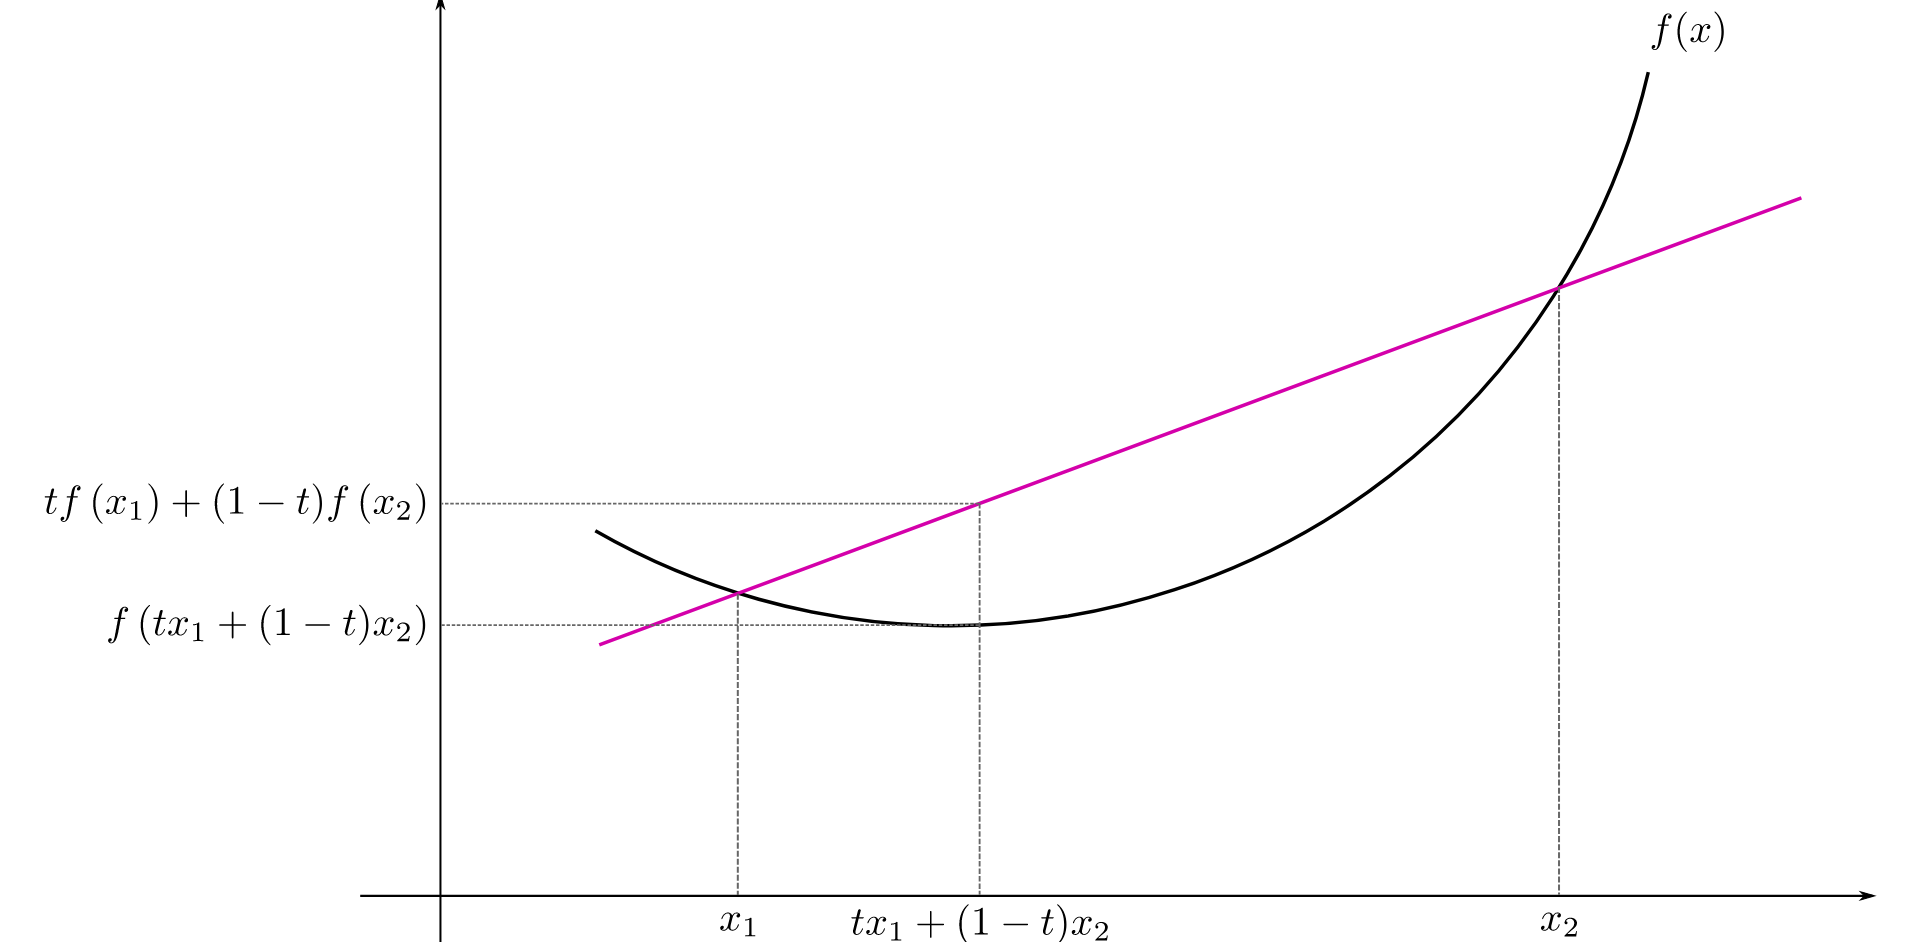
\includegraphics[width=\textwidth]{graph.png}
$x_1 < x_3 <x_2 $ such that $x_3= tx_1+(1-t)x_2$

If $f(x_3) \geq tf(x_1)+(1-t)f(x_2) \rightarrow $ Concave function.

If $f(tx_1+(1-t)x_2) \leq tf(x_1)+(1-t)f(x_2) \rightarrow $ Convex function.

Hence, the above graph is a convex function.

We shall use the concavity property of the log function to obtain the proof for $ H(X) \leq |log \mathcal X| $.

Proof:
$$ H(X)= \sum_{x \in supp(P)} P(x)log\frac{1}{P(x)}$$

Let us assume $\lambda_x$ is another notation for $P(x)$.

$$H(X)= \sum_{x \in supp(P)} \lambda_x log\frac{1}{P(x)}$$

This is a convex combination of $log\frac{1}{P(x)}:x \in supp(P_X)$ as $\sum_{x}P(x)=1$.

$$ H(X) \leq \log \left(\sum_{x \in supp(P_X)}\lambda_x \frac{1}{P(x)} \right) \leq \log |supp(P_x)|$$
$$ \Rightarrow H(X) \leq |\mathcal X |$$

\subsubsection{When is $H(X)$ is $ log|\mathcal X|$?}

When Jensen's inequality is satisfied with equality, i.e. if $f(x)$ is a straight line, but the $\log x$ curve is strictly concave.

Suppose $f(x)$ is strictly concave(or convex) \& $\lambda_1, \lambda_2 \neq 0$ \& $\lambda_1+\lambda_2=1$.

If $f(\lambda_1 x_1 + \lambda_2 x_2)=\lambda_1 f(x_1) + \lambda_2 f(x_2)$, then $x_1=x_2$.

More generally, if $\lambda_i \neq 0 $, $\sum_{i=1}^{n} \lambda_i=1$ and Jensen's inequality holds with equality, then $x_1=x_2\cdots x_n$.

Applying this to $H(X) \leq log|\mathcal X|$, from the previous proof,

$$ H(X)= \sum_{x \in supp(P)} \lambda_x log\frac{1}{P(x)} \leq \log |supp(P_x)| $$
Suppose equality holds, then by the above claim we must have:

$$ \frac{1}{P(X)}= const \quad \forall x \in supp(P_x)$$
$$ \Rightarrow const.\; c= P(x)= \frac{1}{|supp(P_x)|}$$

If $|supp(P_x)|=|\mathcal X|$, $H(X)= \log |supp(P_x)|$. Then $P(X)= \frac{1}{|\mathcal X|}\; \forall x \in \mathcal X$.

We have just proved that $H(X)= \log_2 |\mathcal X|$, this can be true only when $P_x$ is uniform. Thus:

Lemma:
$ H(X)= \log_2 |\mathcal X| $ iff $P_x$ is uniform.

\section{Relative Entropy/ Information Divergence/ Kullback-Leibler Divergence}

Suppose there is a random variable $X$ for which we have two probability distributions $p_x$ \& $q_x$.

Then the RE or ID or KL is defined as:
$$ D(p_X || q_Y):=\sum_{x \in supp(p_x)} p(x)\log \frac{p(x)}{q(x)}$$

($D(p_X || q_Y)$ is a `kind of' a distance measure between distributions p \& q.)

\subsection{Lower limit of relative entropy}
$$ D(p||q)\geq 0$$
Proof:
$$D(p || q)=-\sum_{x \in supp(p_x)} p(x)\log \frac{q(x)}{p(x)}$$
$$ \geq - \log \left(\sum_{x \in supp(p_x)} p(x) \frac{q(x)}{p(x)} \right)$$
$$ \geq - \log\left(\sum_{x \in supp(p_x)} q(x)\right)$$

$$ \geq 0 \quad as \quad \sum q(x) \leq 1$$

\subsection{When is RE equal to zero?}

By applying Jensen's inequality for equality condition.

$$ \frac{p(x)}{q(x)}= const. \; c \qquad \forall x \in supp(p_x)$$
$$ \Rightarrow p(x)=cq(x) \quad \&$$
$$ \sum_{x \in supp(p_x)} p(x)= \sum_{x \in supp(p_x)} cq(x) \forall x \in supp(p_x)$$
These togethermean that $c=1$.
$$\Rightarrow p(x)=q(x) \forall x \in supp(p_x)$$
$$ \Rightarrow D(p||q) \quad iff \quad p_x=q_x$$

\subsection{Upper and lower limits of conditional entropy}

$$ H(X/Y)= \sum_{y \in supp(P_Y)} P_Y(y) \sum_{x \in supp(P_{X/Y})}P_{X/Y}(x/y)\log \frac{1}{P_{X/Y}(x/y)}$$

$$ 0 \leq H(X/Y) \leq H(X)$$

Proof:

$H(X/Y) \geq 0$ is true because $H(X/Y=y)\geq 0$ \& $P(y) \geq 0$.

$$ H(X)-H(X/Y)= \sum_{x \in supp(P_x)}P(x)\log\frac{1}{P(x)}-\sum_{x,y}P(x,y)\log\frac{1}{P(x/y)}$$
$$ =\sum_{x,y}P(x,y)\log\frac{1}{P(x)}-\sum_{x,y}P(x,y)\log\frac{1}{P(x/y)}$$
$$ = \sum_{x,y}P(x,y)\log \left(\frac{P(x/y)}{P(x)}\right)= \sum_{x,y}P(x,y)\log \left(\frac{P(x,y)}{P(x)P(y)}\right)$$

As both $P(x,y)$ \& $P(x)P(y)$ are valid joint distribution of $x,y$. Hence,

$$ H(X)-H(X/Y)= D(P(x,y)||P(x)P(y))$$
$$ \geq 0 \qquad (as\; D(p||q)\geq 0 )$$
$$ \Rightarrow H(X/Y) \leq H(X)$$









\end{document}
